\chapter{The sensorimotor component}\label{ch:robots}

In this chapter the design and architecture of the robots is discussed. The experiments use two small {\sc lego} vehicles, which are controlled by a small sensorimotor board. The robots, including their electronics, were designed at the {\scshape vub ai} Lab. They were constructed such that the configuration of the robots can be changed easily. Sensors may be added or changed and the physical robustness of the robots has improved through time. In some experiments they {\it are} changed substantially, but in most experiments the robots remain the same.

The robots are controlled by a specialised sensorimotor board, the {\sc smbii}\footnote{Read as {\sc smb}-\oldstylenums{2}.} \citep{vereertbrugghen:1996}. The sensorimotor board connects the sensory equipment with the actuators in such a way that the actuators and sensor readings are updated 40 times per second. The actuators respond to sensory stimuli, where the response is calculated by a set of ``parallel'' processes. These processes are programmed in the {\em Process Description Language} (\textsc{pdl}), which has been developed at the {\scshape vub ai} Lab as a software architecture to implement behaviour-oriented control \citep{steels:1994b}. 

The outline of the experiments is discussed in \chapref{ch:lg}; this chapter is concentrated on the physical set-up of the robots and their environment in the different experiments. The robots' environment is presented in \sectref{s:robots:envir}. \sectref{s:robots:robots} discusses the physical architecture of the robots. Section \ref{s:robots:PDL} discusses the Process Description Language. 

\section{The environment}\label{s:robots:envir}

The environment that has been used for the experiments in the past varied across some of the experiments. The environment in early experiments \citep{steelsvogt:1997,vogt:1998b,vogt:1998a} had different light sources than the current environment. Furthermore, the size of the environment shrinked from $5\cdot 5 m^2$ to $2.5\cdot 2.5 m^2$. In the current environment there are four different white light sources, each placed at a different height (\figref{f:robots:envir}).

These white light {\scshape (wl)} sources (or light sources for short) all emit their light from black cylindrical boxes with  small slits. The light sources are halogen lights and each box now has a height of 22 cm, a diameter of 16 cm and 3 horizontal slits. Each slit has its centre at a height of 13 cm (measured from the bottom of the box) and is 0.8 cm wide. Although the different slits are intersected by a bar, they can be approximated to be one slit.

The boxes are placed such that the height of the slit varied per light source. The four different heights are distributed with a vertical distance of 3.9 cm. In one experiment the difference in height was changed to 2.9 cm. The robots were adjusted to this environment (or vice versa) so that the light sensors were placed at the same height as the centre of the slits.

\begin{figure}
	\centerline{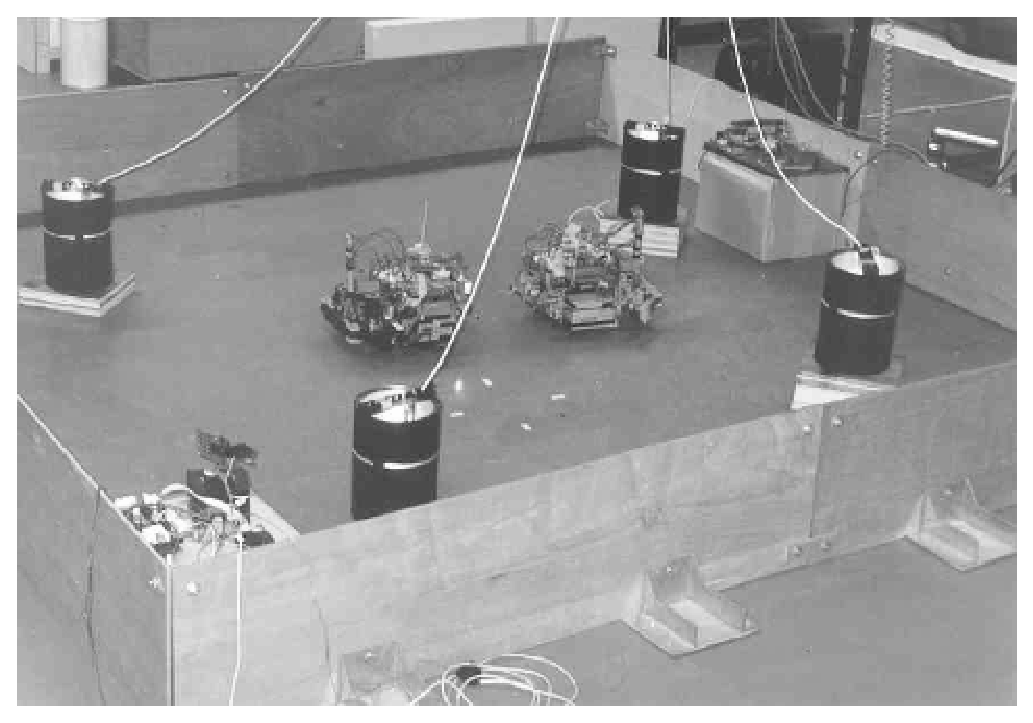
\includegraphics[width=8cm]{robots//environment.eps}}
	\caption{The robots in the environment as is used in the experiments.}
	\label{f:robots:envir}
\end{figure}

\section{The robots}\label{s:robots:robots}

\enlargethispage{1\baselineskip}
In the experiments two {\sc lego} robots as in \figref{f:robots} are used. Each robot has a set of sensors to observe the world. These sensors are low-level. They can only detect the intensity of light in a particular frequency domain. Other low-level sensors are used to control the robots in their movement. The sensors are connected to a dedicated sensorimotor board, the so-called {\sc smbii}. On the {\sc smbii} all sensors are read at a rate of 40 {\scshape h}{\scriptsize z}. The sensor readings are processed according to the software, written in {\sc pdl} (see next section). After the sensors have been processed the {\sc smbii} outputs the actuator commands and sends its appropriate signals to the actuators. The robots are powered by a re-chargeable nickel--cadmium battery pack as used in portable computers.

In this section the set-up of the sensors and actuators of the robots are discussed first. Secondly the architecture of the {\sc smbii} is discussed briefly.

\begin{figure}
	\centerline{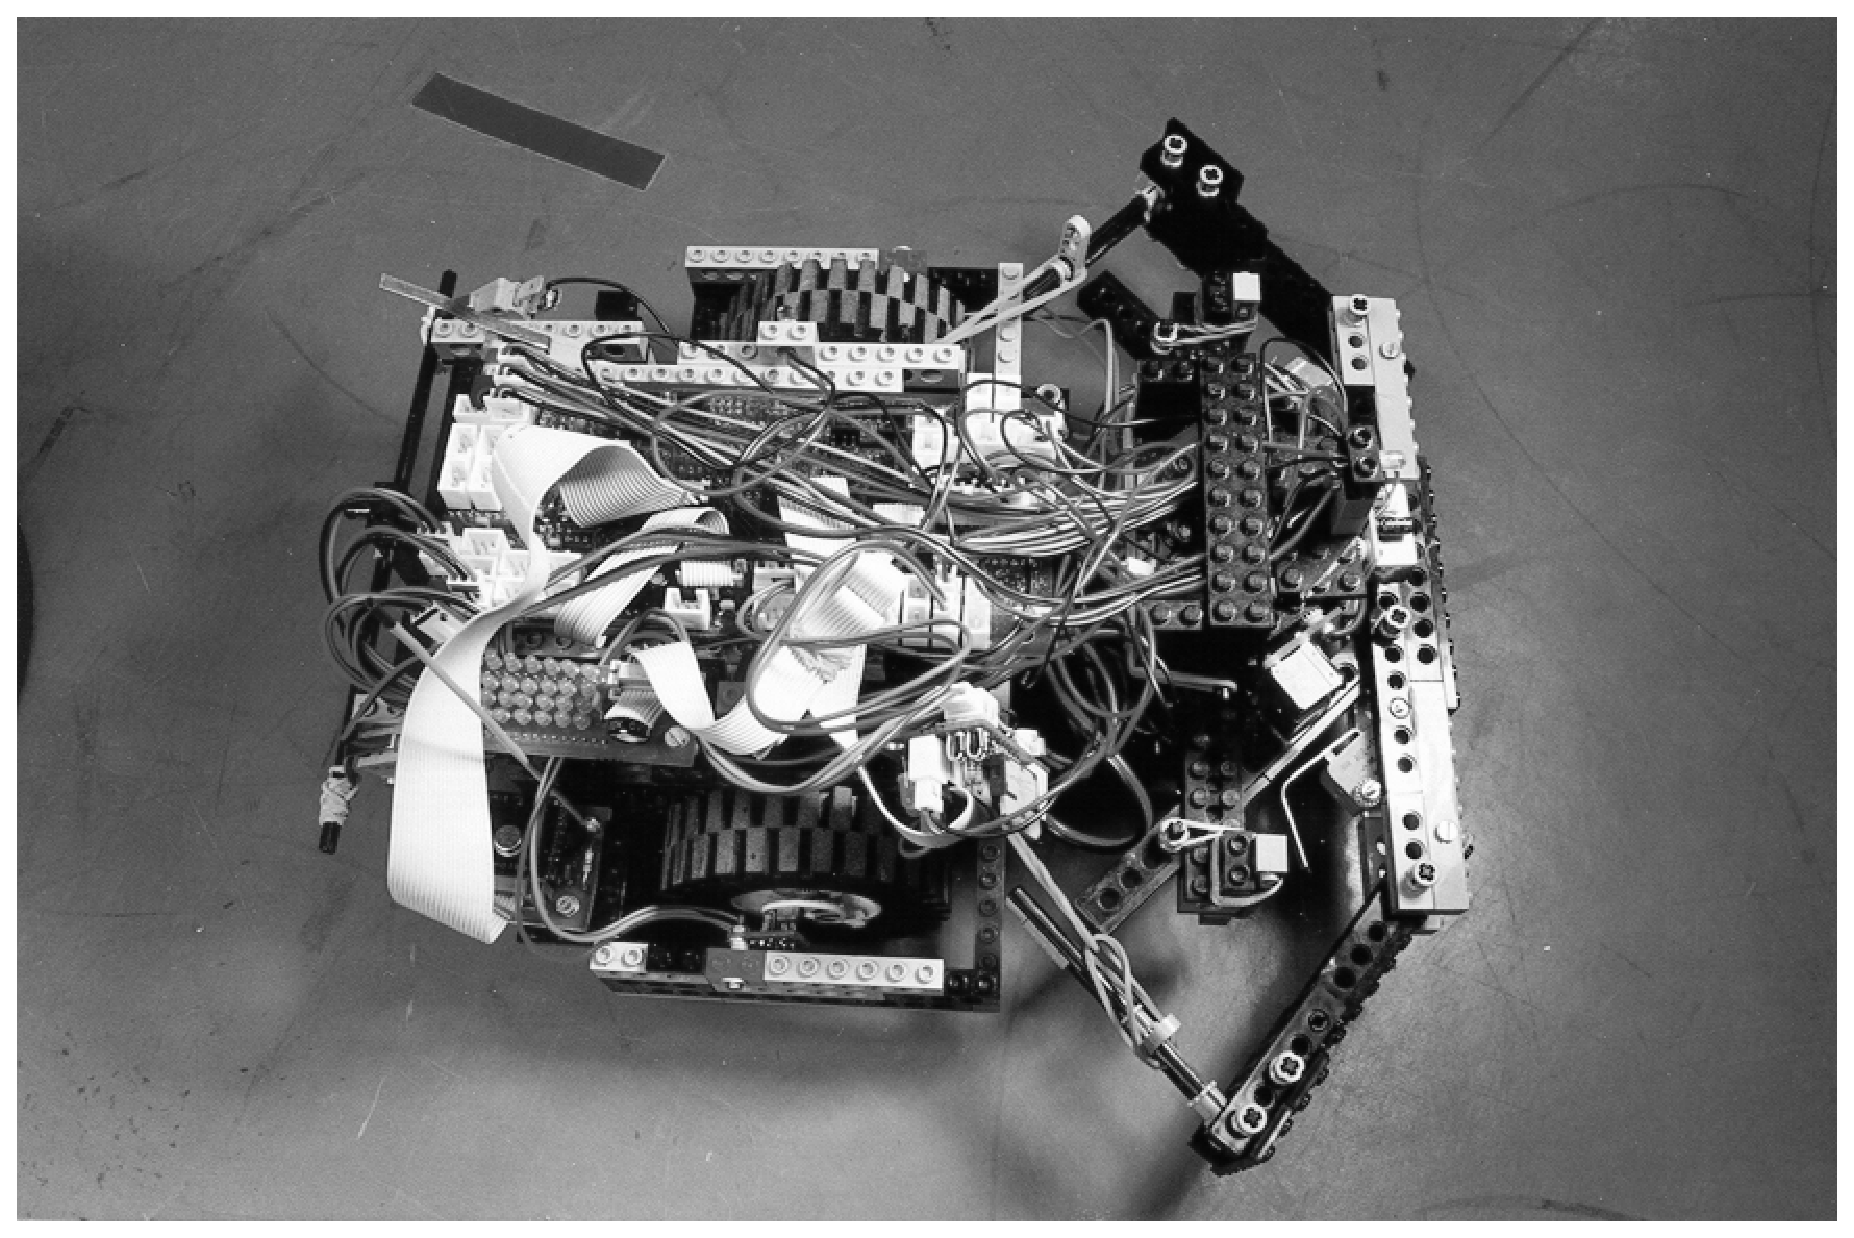
\includegraphics[width=8cm]{robots//robot.eps}}
	\caption{One of the {\sc lego} robots used in the experiments.}
	\label{f:robots}
\end{figure}
\subsection{The sensors and actuators}\label{s:robots:sensors}

\begin{figure}[t]
\centerline{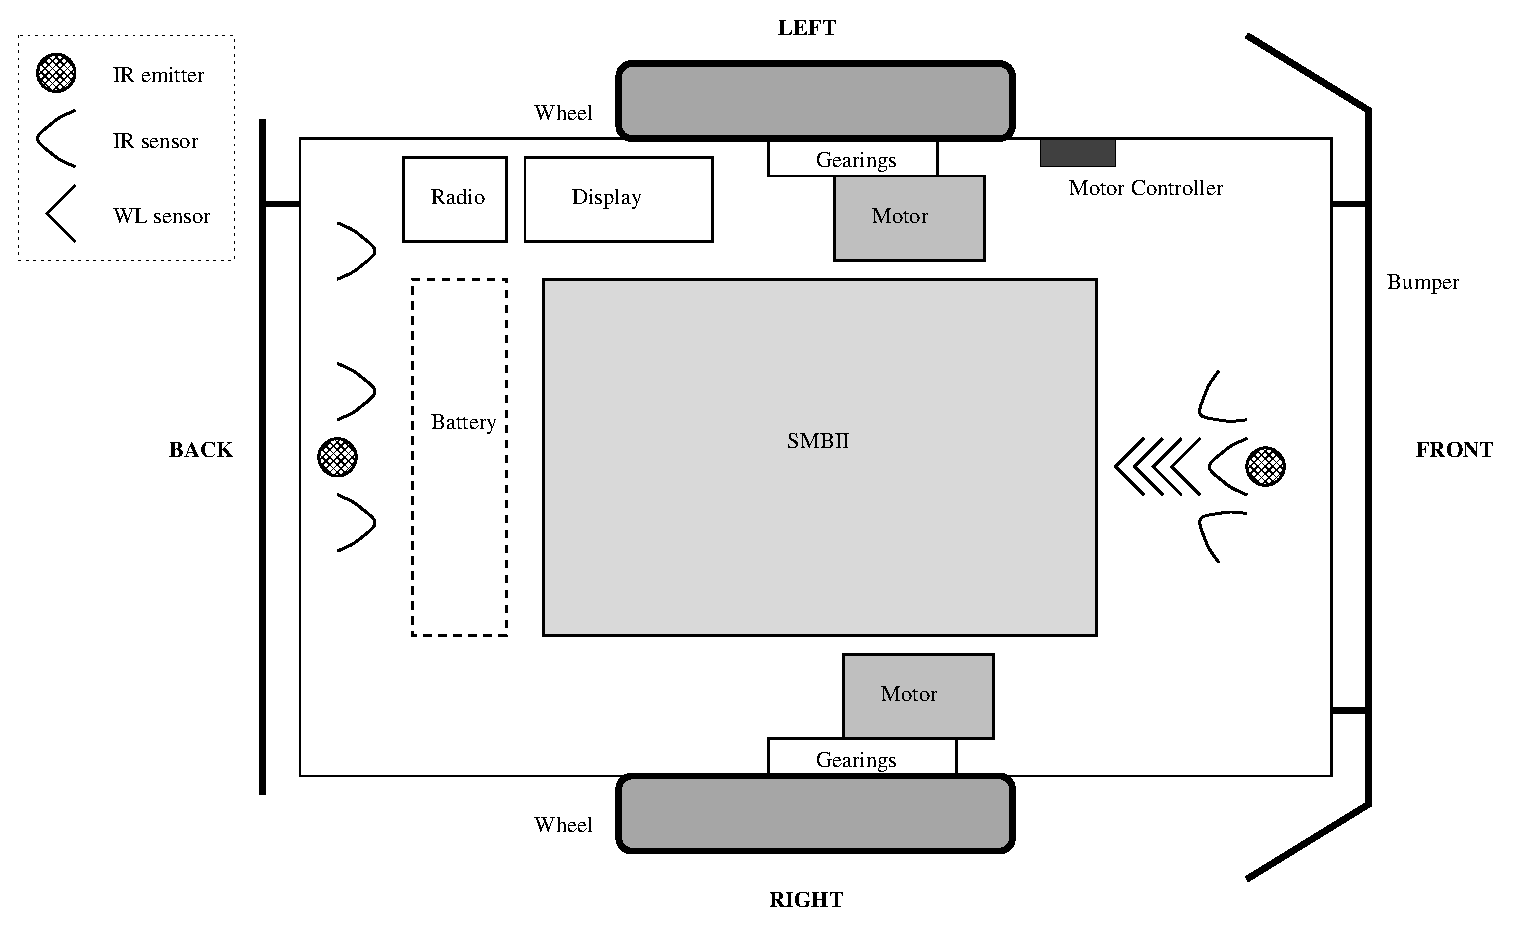
\includegraphics[width=8cm]{robots//schema_robots_exp2.eps}}
\caption{A schematic overview of the basic set-up of the robots that are used in the experiments.}
\label{f:robots:robots_general}
\end{figure}

The robots in all experiments have a set-up like shown schematically in \figref{f:robots:robots_general}. The sensory equipment consists of four binary bumpers, three infrared {\scshape (ir)} sensors and a radio link {\em receiver}. The radio link is a module that also has a radio link {\em transmitter}, which is classified as an actuator. The infrared sensors are part of the infrared module, which also consists of an actuator: the infrared transmitter. Two independent motors complete the actuator set-up. All sensors and actuators are connected to the {\sc smbii}, which is powered by a battery-pack. The battery-pack also powers the motor-controller. The motor-controller, controlled by the {\sc smbii} controls the motors. The motors are connected to the wheels via a set of gears. Finally there are four white light sensors that are responsible for the perception.

Below a more detailed description of the most important sensors and actuators are given. 


\begin{description}
\item[The bumpers] The robots have four bumpers that are used for touch based obstacle avoidance; two on the front and two on the back of the robot, both left and right. Each bumper is a binary switch: when it is pressed it returns $1$, else it returns $0$. The bumpers have a spanning construction of {\sc lego} (see \figref{f:robots:front} and \ref{f:robots:radiolink}). If a robot bumps with this construction into an obstacle. The program can then react on the sensed collision.
\item[The infrared module] Whereas the bumpers are simple binary sensors, the infrared module \figref{f:robots:front} is more complex. The infrared module consists of infrared emitters and sensors. The emitters are light emitting diodes emitting infrared. The infrared sensors themselves are sensors that can be found in e.g. television sets. They detect light at infrared wavelengths and send a signal to the {\sc smbii} that is proportional to the intensity of the infrared. The sensors are mounted such that they can discriminate infrared coming from the left, centre and right sides in front of the robot. The sensors are not calibrated in the sense that one can calculate the exact angle from where the infrared is coming or from what distance. Also the  positions of the sensors are not exactly symmetric, due to some physical limitations of the sensors and the {\sc lego} construction. \citet{vogt:1997} discusses some practical problems concerning the modulation and characteristics of the infrared module in detail.

\item[The radio link] The radio link module is a transmitter/receiver device designed to connect with the {\sc smbii} (see \figref{f:robots:radiolink}). The module is a Radiometrix {\scshape bm}-\oldstylenums{433}{\scshape f} module with {\scshape rx} (receive) and {\scshape tx} (transmission) connections. The module can send up to 40 Kbit/s, but is used at 9.6 Kbit/s. 

Every clock cycle of the {\sc smbii} a packet of messages can be sent. A packet can consist of a maximum of 31 messages each up to 127 bytes long. A message has a transmission {\scshape id} and an destination address, which define the sender and receiver(s) of the message.  It also has a bit defining the reliability of the transmission; this bit has to be set to {\it unreliable}, i.e. to $0$, because the reliability protocol has not been implemented in the radio link kernel. This has the consequence that if a message is sent, it is not sure if the message arrives at its destination. But {\em when} it arrives, the message arrives error-less. About 5~\% of the messages sent do not arrive at their destination.

This unreliability has some technical impacts on the experiments. Since data logging, recording and communication passes through the radio link, not all information is received. Filters had to written to find out whether all data was logged and if not, part of the data would be unreliable and should therefore be discarded. It is beyond the scope of this dissertation to go into the details of such filters here. For the purpose  of the book it is assumed that the radio transmission is reliable.

\item[The motor controller and the motors] The motor controller is a device that transforms and controls motor commands coming from the {\sc smbii} into signals that are sent to the standard {\sc lego dc} motors. Each robot has two independent motors. So, in order to steer the robot, one has to send a (possibly different) signal to each motor.

\item[Gearing] The motors are not directly connected to the wheels. They are connected to the wheels with a set of gears (see \figref{f:robots:bottom}). The wheels are placed such that they form an axis approximately through the centre of the robot so that it can rotate around this point. A third small caster-wheel is used to stabilise the robot. 

\index{sensors light|(}
\item[The light sensors] The white light sensors are the most crucial sensors in the experiments. This is because they are used for the perception of the analogue signals that the robots are supposed to ground. Each robot has four white light sensors stacked on top of each other. The sensors have a vertical distance of 3.9 cm between each other. Each sensor is at the same height as a light source (\figref{f:robots:front}). 

The light sensors were calibrated such that the characteristics of all sensors are roughly the same. \figref{f:robots:calibration} shows the characteristics of the calibrated light sensors as empirically measured for the experimental set-up. On the x-axis of each plot the distance of the robot to the light source is given in centimetres; the y-axis shows the intensity of the light in {\sc pdl} values. {\sc pdl} scales the light sensors between 0 and 255, where 0 means no detection of light and 255 means maximum intensity. The calibration of each sensor is done while it was exposed to a corresponding light source. A sensor is said to {\em correspond} with a light source when it has the same height. The complete figure shows the characteristics of the two robots $r0$ and $r1$, each with four sensors ($s0 \ldots s3$).
\index{correspondence}

It is notable that for light source $L0$ the characteristics of sensor $s3$ is high at the beginning (\figref{f:robots:calibration} (a) and (e)). This is because for the lowest light source $L0$, sensor $s3$ is higher than the top of the box, which is open. At a larger distance the light coming from the top of this box cannot be seen. 

It is clear that all characteristics are similar. The sensor that corresponds to a light source detects high intensities at short distances and low values at larger distances. From 0.6 m other sensors start detecting the light source as well. This is because the light coming from the slit does not propagate in a perpendicular beam, but is diverging slightly. It is important to note that corresponding light sensors are calibrated to read the highest intensities between 0 and 1.2 m. The shape of the plots are like they would have been expected from the physics rule that the intensity $I \sim \frac{1}{r^2}$, where $r$ is the distance to the light source.

It is noteworthy that each sensor detects noise that comes mainly from ambient light.
\end{description}

\begin{figure}
	\centering
	\subfigure[Front]{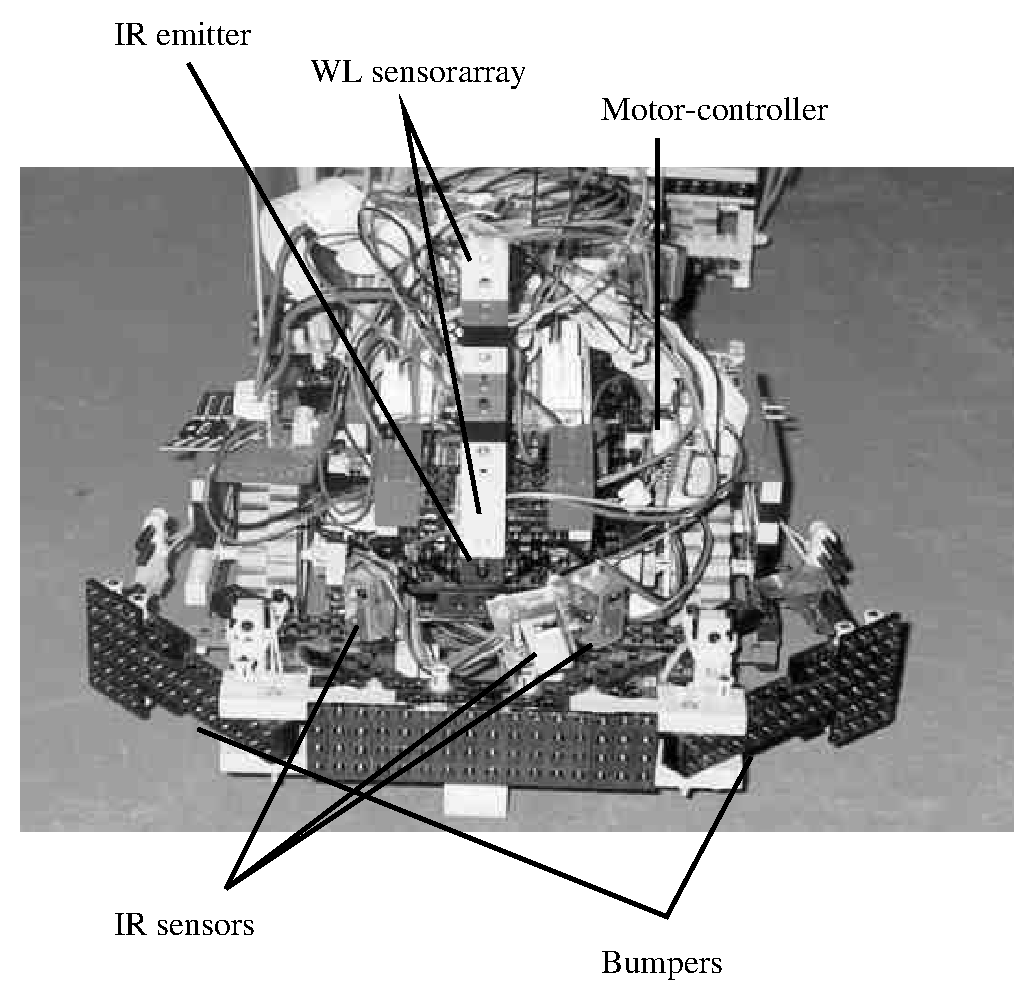
\includegraphics[width=8cm]{robots//front1.eps}\label{f:robots:front}}\\
	\subfigure[Back]{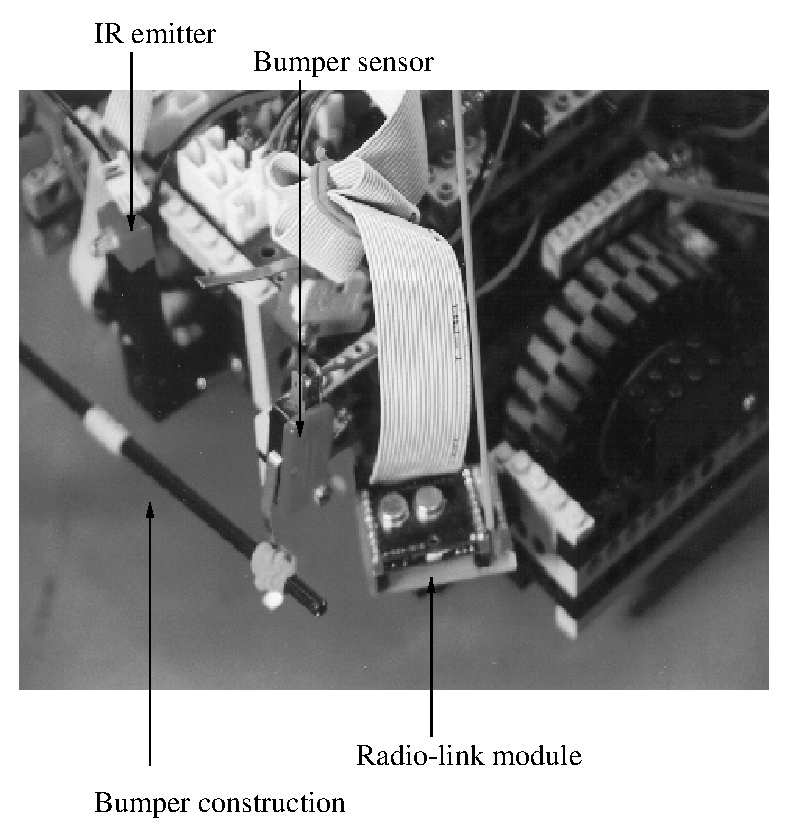
\includegraphics[width=8cm]{robots//radio.eps}\label{f:robots:radiolink}}
\end{figure}
\begin{figure}
	\centering
	\subfigure[Bottom]{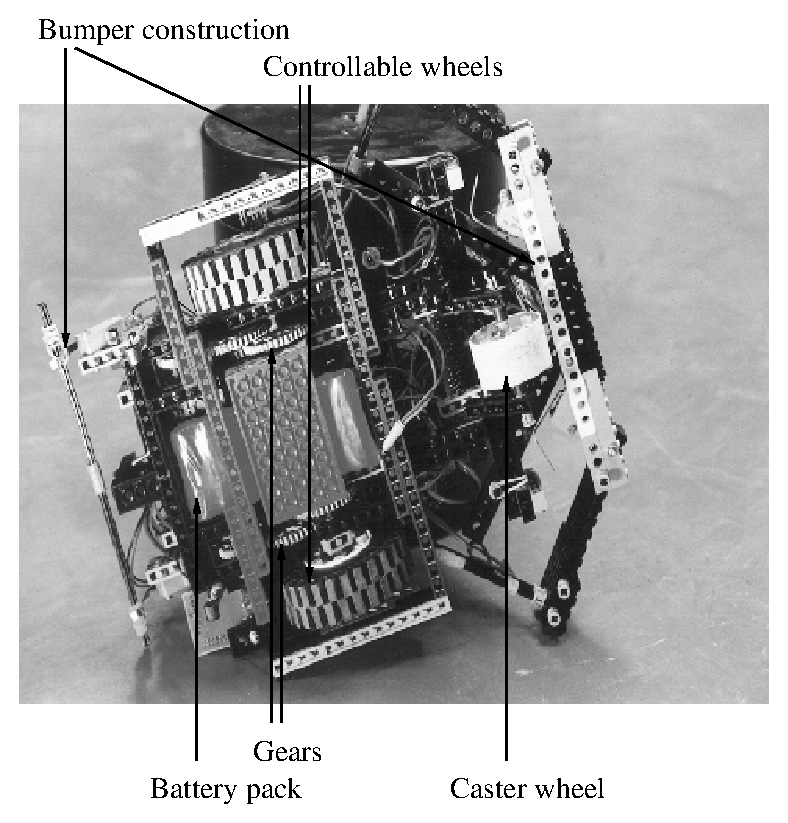
\includegraphics[width=8cm]{robots//bottom1.eps}\label{f:robots:bottom}}
	\caption{Several close ups of one of the robots. Figure (a) shows the front side of the robot. The bumper construction can be seen. The perceptual sensor array consisting of 4 light sensors, the infrared sensors and the infrared emitter are also visible. The radio link module can be seen in (b) as well as a part of the bumper construction on the back. Figure (c) shows the bottom of the robot. We see the wheels, gearing and the battery pack. Also a good view is seen of the bumper constructions.}
\end{figure}

The robots are also equipped with sensors and actuators that are used for interfacing the robot with the experimenter. It has for instance a serial port for connecting the robot to a {\scshape pc}, a display with 64 \textsc{leds}, a pause button, an on/off switch, etc. Since these sensors are not vital for the behaviour of the robots, they are not discussed in more detail here. 


\begin{figure}
\centering
\subfigure[r0, L0]{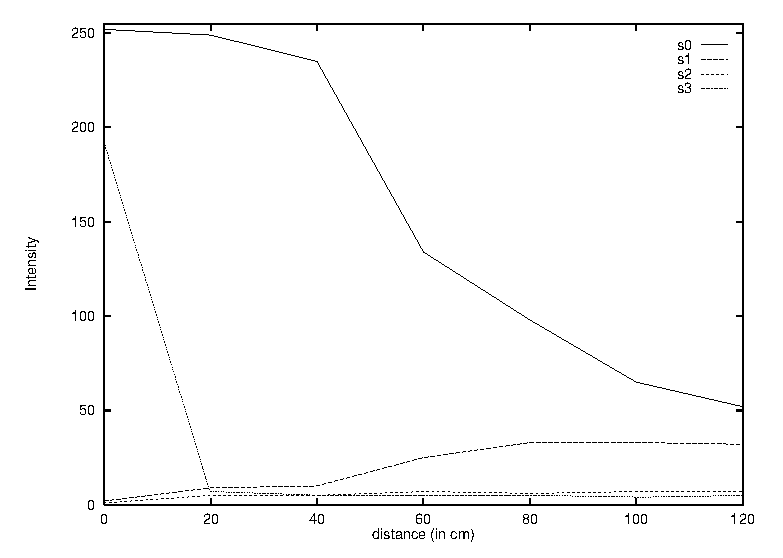
\includegraphics[width=5.5cm]{robots//char_sens_r0s0.eps}}
\subfigure[r0, L1]{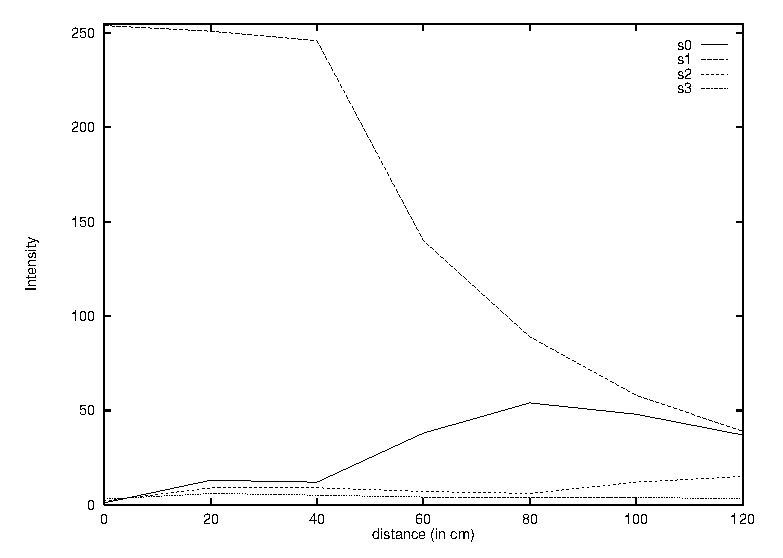
\includegraphics[width=5.5cm]{robots//char_sens_r0s1.eps}}\\
\subfigure[r0, L2]{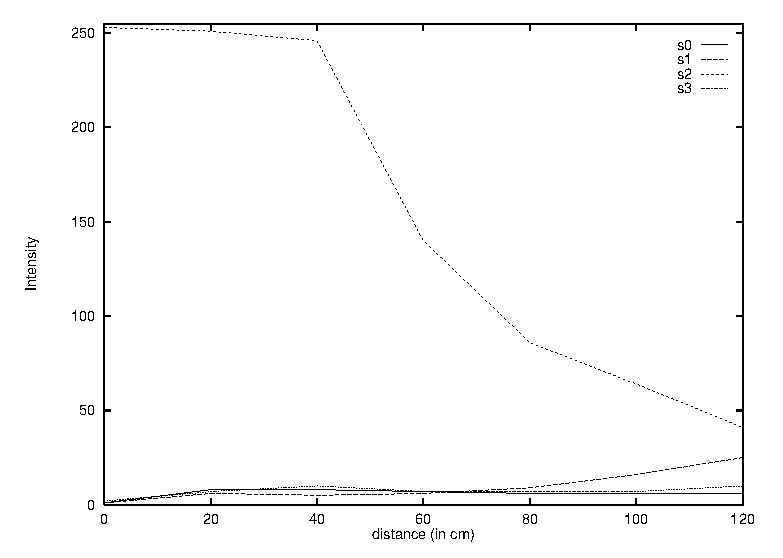
\includegraphics[width=5.5cm]{robots//char_sens_r0s2.eps}}
\subfigure[r0, L3]{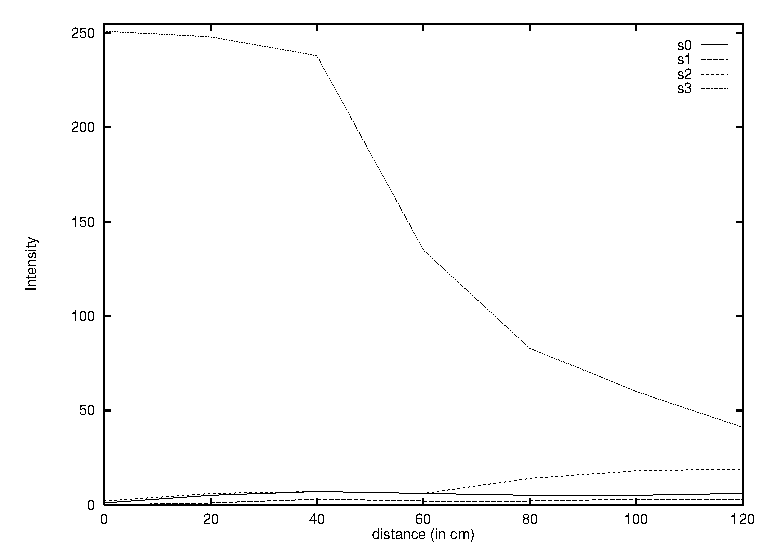
\includegraphics[width=5.5cm]{robots//char_sens_r0s3.eps}}
\end{figure}

\begin{figure}
\centering
\subfigure[r1, L0]{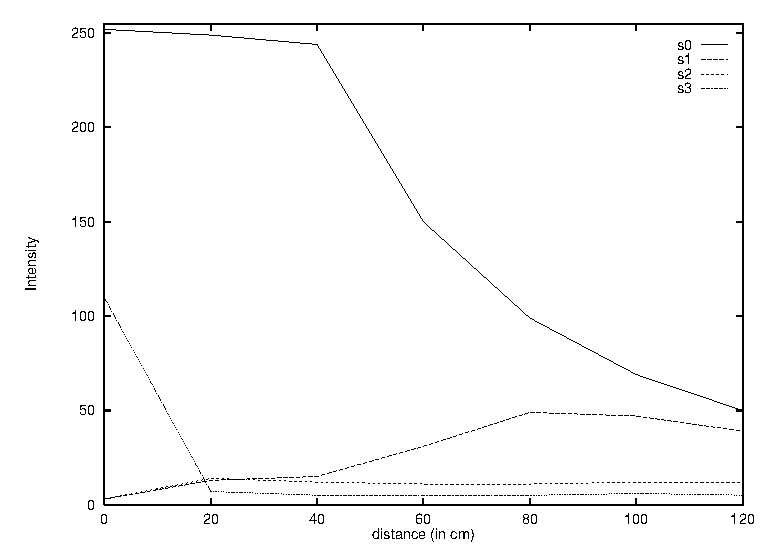
\includegraphics[width=5.5cm]{robots//char_sens_r1s0.eps}}
\subfigure[r1, L1]{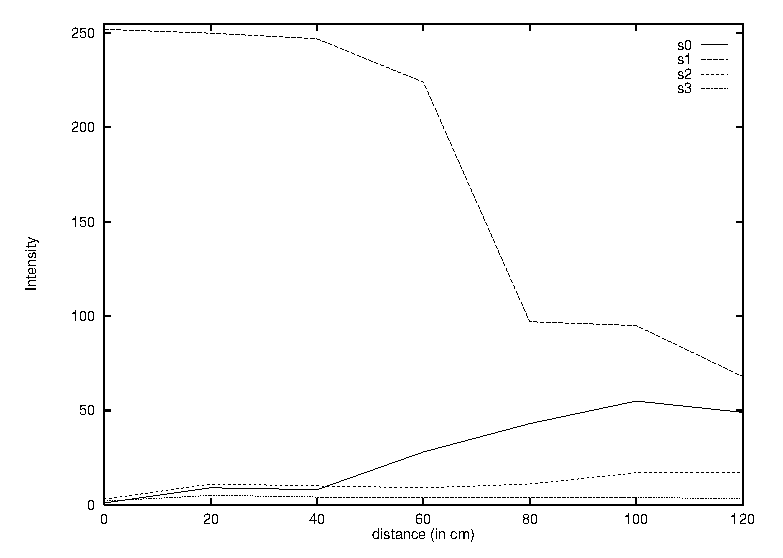
\includegraphics[width=5.5cm]{robots//char_sens_r1s1.eps}}\\
\subfigure[r1, L2]{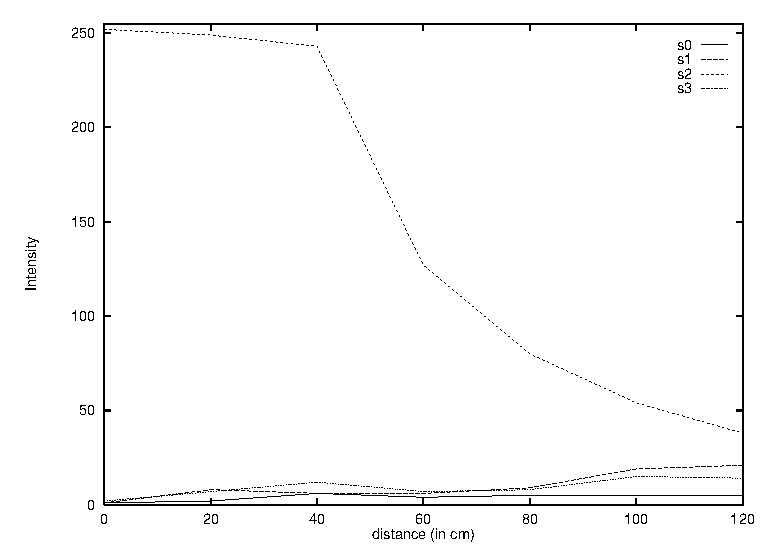
\includegraphics[width=5.5cm]{robots//char_sens_r1s2.eps}}
\subfigure[r1, L3]{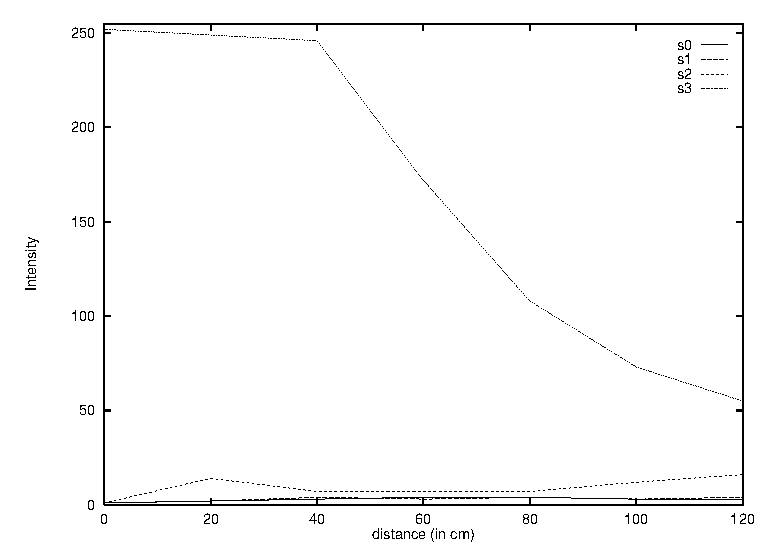
\includegraphics[width=5.5cm]{robots//char_sens_r1s3.eps}}
\caption{The characteristics of the calibrated light sensors as empirically measured for the experimental set-up when exposed to light sources $L0 - L3$. Plots (a) -- (d) show the of robot $r0$ and plots (e) -- (h) show them for $r1$. The distances are measured from the front of the robots to the boxes. Actual distances from source to sensor are 12 cm further.}
\label{f:robots:calibration}
\end{figure}

\index{sensors light|)}

\bigskip\noindent
This subsection introduced the sensorimotor equipment that the robot carries in the experiments as discussed throughout this book. The next subsection discusses the sensorimotor board in some more detail.

\subsection{Sensor-motor board II}\label{setup:smbii}


The computing hardware of the robots is a sensorimotor board, called the {\sc smbii}, which is developed at the {\scshape vub ai} Lab by Dany \citet{vereertbrugghen:1996}. It consists of an {\scshape add-on smb-{\oldstylenums 2} board} and a Vesta Technologies {\scshape sbc}\oldstylenums{332} micro controller board.

\begin{figure}
\centering
\subfigure[Vesta board]{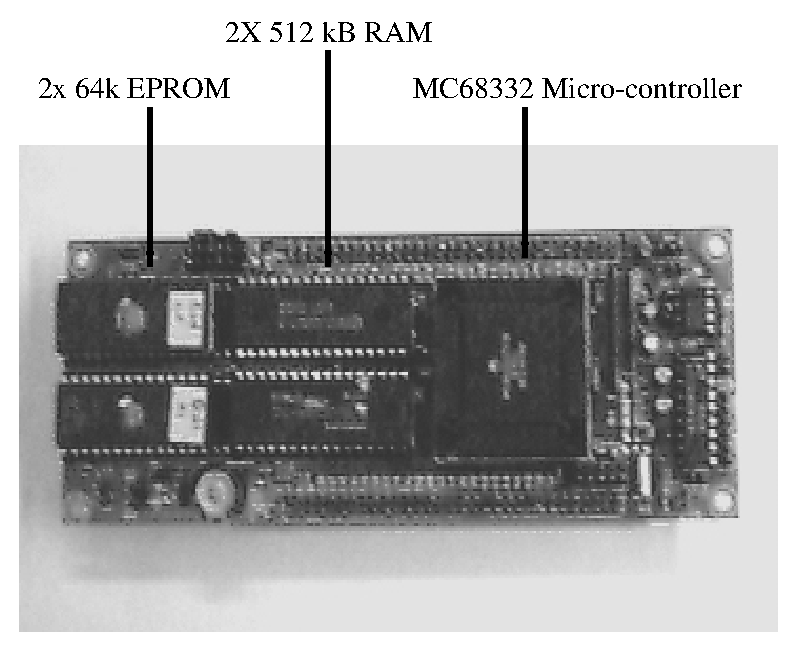
\includegraphics[width=.45\textwidth]{robots//vesta.eps}\label{f:vesta}}
\subfigure[\textsc{smb}-{\oldstylenums 2} add-on]{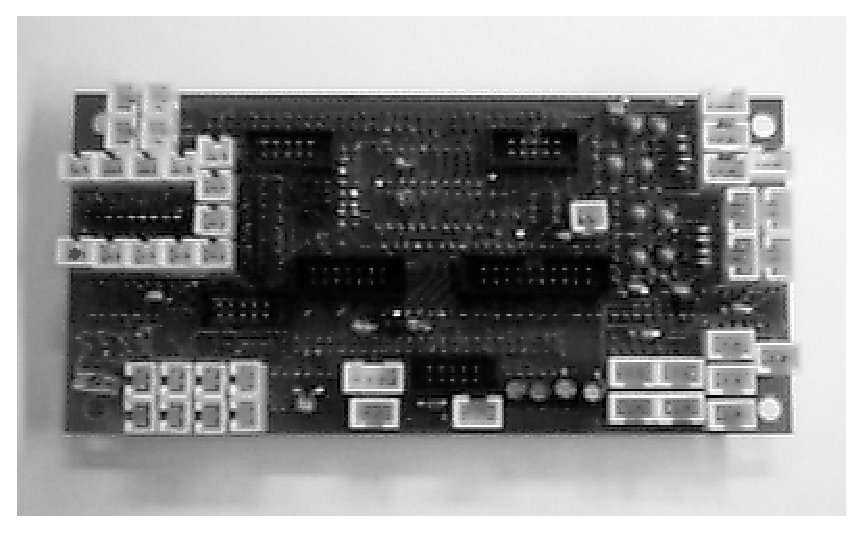
\includegraphics[width=.45\textwidth]{robots//smb2.eps}\label{f:smbii}}
\caption{The two components of the {\sc smbii} board: (a) the Vesta Technologies {\scshape sbc}\oldstylenums{332} micro controller board, and (b) the add-on {\sc smb}-{\oldstylenums 2} sensorimotor board.}
\end{figure}

The Vesta board (see \figref{f:vesta}) contains a Motorola \textsc{mc}\oldstylenums{68332} microcontroller, {128} {\footnotesize k}{\scshape b} {\scshape rom} and {1} {\scshape mb ram}.\footnote{In the original version of the {\sc smbii} there were only {256} {\scriptsize k}{\scshape b} {\scshape ram} \citep{vereertbrugghen:1996}.} The board's micro-controller runs at 16.78 {\scshape mh}{\footnotesize z} at 5 Volt and everything is powered by a pack of rechargeable nickel--cadmium batteries.

The add-on {\sc smb}-{\oldstylenums 2} board (\figref{f:smbii}) contains several {\scshape i/o} chips, bus controllers and connectors. The {\sc smbii} low-level program is run on the kernel and it can interface a user program written in any language as long a the kernel calls are written in \textsc{c}  \citep{vereertbrugghen:1996}. The program that is run on the {\sc smbii} for these experiments is written in the Process Description Language {\sc pdl}. 
\index{SMBII}

\section{The Process Description Language}\label{s:robots:PDL}\label{s:robots:pdl}
\index{PDL|(}
\index{Process Description Language|see{PDL}}

The robots are programmed in the so-called Process Description Language \citep{steels:1992,steels:1994a,steels:1994b}. {\sc pdl} is designed as a framework for designing software for autonomous agents according to the behaviour-oriented control. 

\index{phototaxis|(}
In {\sc pdl} one can decompose a behaviour system in a set of dynamical processes. For instance, one can decompose the behaviour of {\scshape phototaxis} (i.e. moving towards a light source) into two dynamical processes: (1) moving forward and (2) orienting towards the light. {\sc pdl} is designed to implement parallel processes that are virtually evaluated simultaneously to output a summated response. So, suppose there are the two parallel processes (1) and (2) that are evaluated  simultaneously. And suppose further that the output of the two processes are summated to give a motor response. Then the emergent behaviour is phototaxis. 

\begin{figure}
\centerline{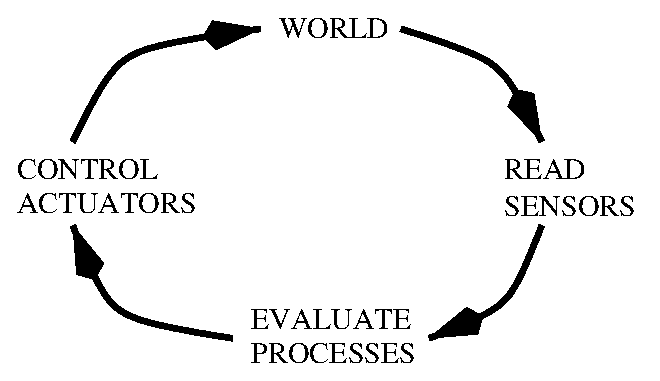
\includegraphics[width=.5\textwidth]{robots//pdlcycle.eps}}
\caption{The way that {\sc pdl} interacts with the world via a robot. Every $\frac{1}{40} s$ {\sc pdl} is going through a cycle as shown in the figure.}
\label{f:pdlcycle}
\end{figure}

{\sc pdl} cycles the process of {\scshape reading sensors}, {\scshape evaluate processes} and {\scshape control actuators} (\figref{f:pdlcycle}). During a {\sc pdl} cycle a robot reads the sensors to detect the current state of a robot in the world. These sensor readings are evaluated by processes that are defined in the software as explained below. The processes output commands to activate the actuators. These actuators in turn change the state of the world. Such a cycle is processed at 40 \textsc{h}{\footnotesize z}, so 40 {\sc pdl} cycles take 1 second. Throughout the book the basic time unit is a {\sc pdl} cycle ($\frac{1}{40} s$).

The initial implementation of {\sc pdl} was written in {\sc lisp}, the currently used version is implemented in {\sc ansi-c}. It can compile both the specialised {\sc pdl} syntax and {\sc ansi-c} commands within its architecture. The {\sc pdl} architecture has as its basic symbolic units so-called \texttt{quantities}. A quantity is a \texttt{struct} type that has a {\sc name}, a {\sc value}, an {\sc upper bound}, a {\sc lower bound} and an {\sc initial value}. Each quantity can be connected to a serial port, interfacing the program with the physical sensors and actuators. Each type of sensor and actuator is defined within the operating system of the {\sc smbii}. The radio module has its own interface, but can be called with a {\sc pdl} command. The most important parts of a {\sc pdl} program are the {\em processes}. Each time a {\sc pdl} program is compiled, a network of processes is build up. The following example of phototaxis shows how this is done.

The example implements two behaviours: (1) {\scshape infrared orientation} and (2) {\scshape infrared phototaxis}. In infrared orientation, the goal of the robot is to orient itself in the direction of an infrared source without approaching the source.\footnote{In the experiments the robots themselves are infrared sources.} It is implemented using only one dynamic process called {\scshape taxis}. With infrared phototaxis the goal of a robot is to approach the infrared source. It is implemented with an additional process that causes a robot to try to move at a default speed. 

After declaration, the quantities have to added to the system as follows:

\begin{lstlisting}
add_quantity(LeftFrontIR,''LeftFrontIR'',255.0f,0.0f,0.0f);
add_quantity(RightFrontIR,''RightFrontIR'',255.0f,0.0f,0.0f);
add_quantity(LeftMotor,''LeftMotor'',100.0f,-100.0f,0.0f);
add_quantity(RightMotor,''RightMotor'',100.0f,-100.0f,0.0f);
\end{lstlisting}

\begin{figure}
\centerline{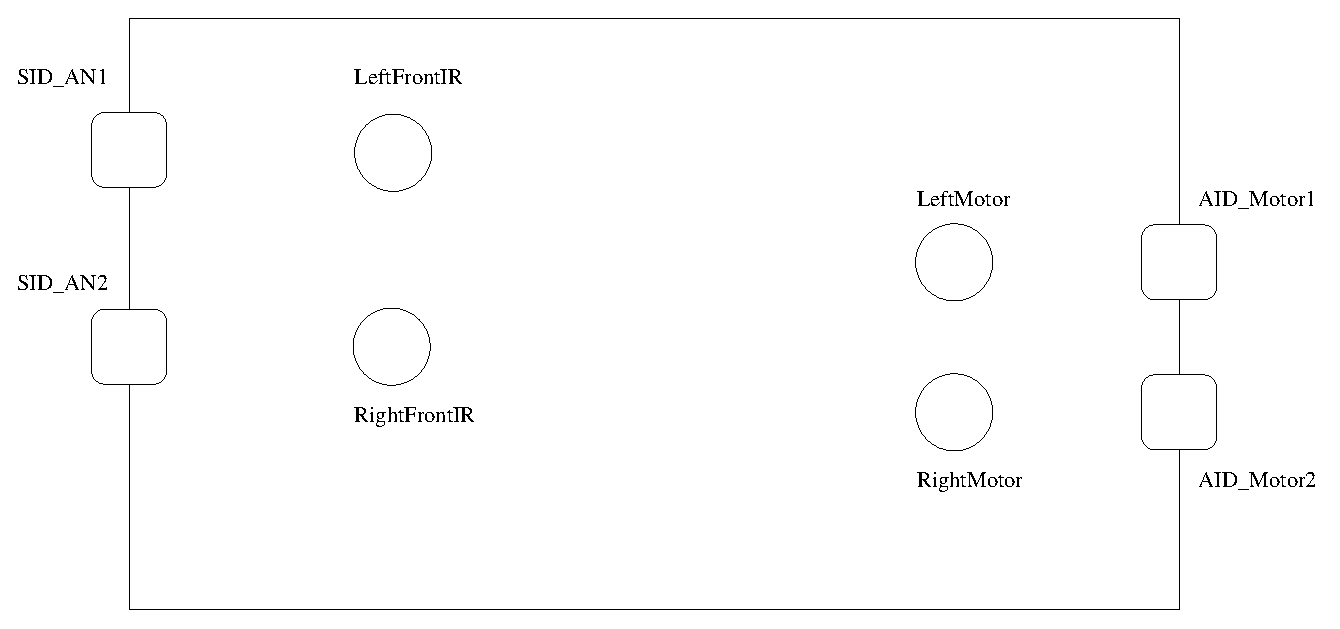
\includegraphics[width=9cm]{robots//pdl_networka.eps}}
\caption{The construction of a {\sc pdl} network. The program has serial ports \mbox{{\sc sid\_an{\oldstylenums 1}}} and {\sc sid\_an{\oldstylenums 2}} for analogue sensory input. Ports {\sc aid\_motor{\oldstylenums 1}} and {\sc aid\_motor{\oldstylenums 2}} are serial ports for the motors. The network consists of the quantities \texttt{LeftFrontIR}, \texttt{RightFrontIR}, \texttt{LeftMotor} and \texttt{RightMotor}.}
\label{f:robots:pdl_networka}
\end{figure}
\noindent
The function \texttt{add\_q} adds the quantity \texttt{LeftFrontIR} to the network, an upper bound of \texttt{255.0f} (where \texttt{f} stands for ``float''), a lower bound of \texttt{0.0f} and an initial value of \texttt{0.0f}. Likewise the quantities \texttt{RightFrontIR, LeftMotor} and \texttt{RightMotor} were added, see \figref{f:robots:pdl_networka}. The upper and lower bound of the motors are 100.0 and \textminus 100.0, respectively. If, mathematically, an upper or lower bound would be exceeded, {\sc pdl} sets the quantity-value to its upper or lower bound. The next step is to connect the quantities to the serial ports of the {\sc smbii}, which are connected to the sensors and actuators.


\begin{lstlisting}
add_connection(SID_AN1,LeftFrontIR);
add_connection(SID_AN2,RightFrontIR);
add_connection(AID1_Motor,LeftMotor);
add_connection(AID2_Motor,RightMotor);
\end{lstlisting}

\begin{figure}
\centerline{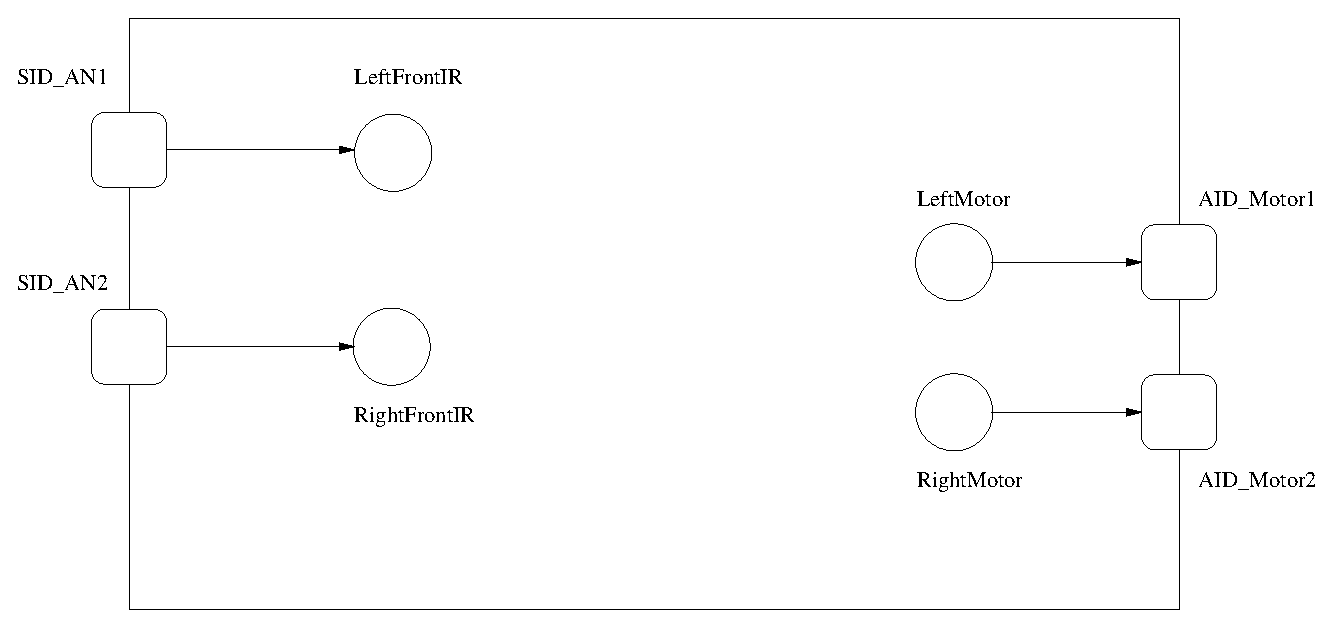
\includegraphics[width=9cm]{robots//pdl_networkb.eps}}
\caption{This is the {\sc pdl} network after the quantities are connected with the serial ports.}
\label{f:robots:pdl_networkb}
\end{figure}

Now the network looks like in \figref{f:robots:pdl_networkb}. The above is part of the initialisation. Another step of the initialisation is to add processes to the network:

\begin{lstlisting}
add_process(Taxis,''Taxis'');
add_process(TowardsDefault,''TowardsDefault'');
\end{lstlisting}

\begin{figure}
\centerline{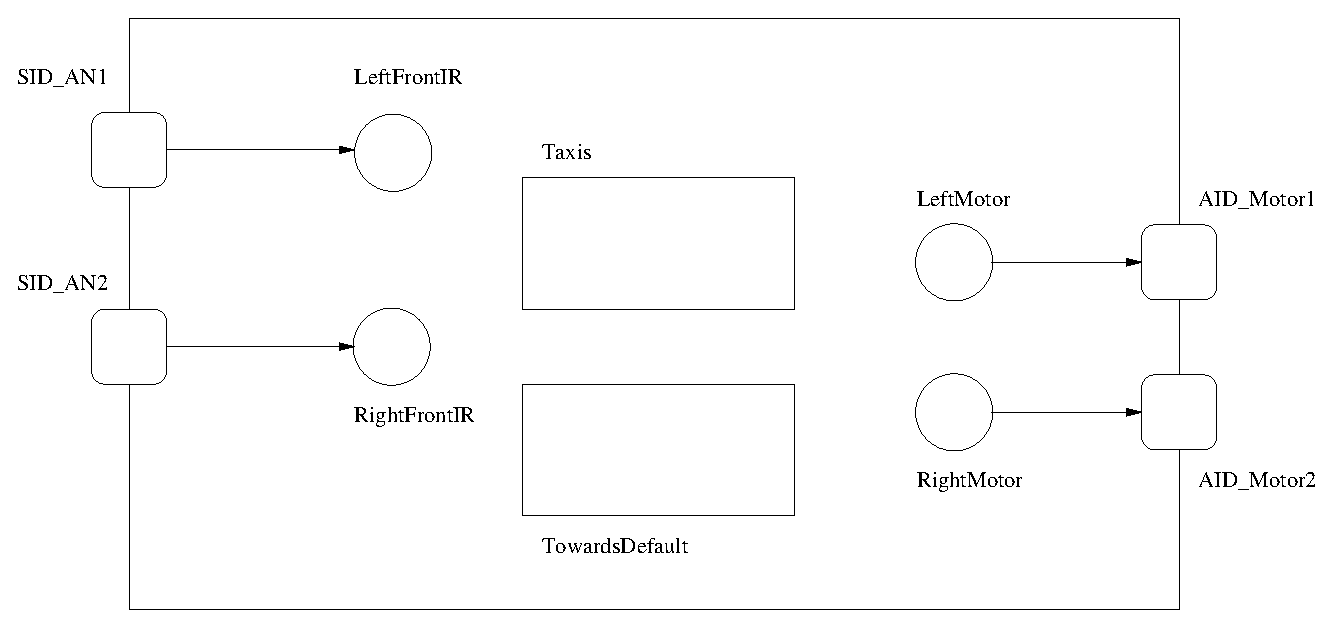
\includegraphics[width=9cm]{robots//pdl_networkc.eps}}
\caption{This is the {\sc pdl} network after the processes \texttt{Taxis} and \texttt{TowardsDefault} are added.}
\label{f:robots:pdl_networkc}
\end{figure}


This leads to the network as shown in \figref{f:robots:pdl_networkc}. To couple the sensors with the actuators, the processes have to be defined. The process {\ttfamily Taxis} causes the robot to orient towards an infrared light source.


\begin{lstlisting}
void Taxis()
{
  D=value(RightFrontIR)-value(LeftFrontIR);
  add_value(LeftMotor,C*F(D)*D));
  add_value(RightMotor,-C*F(D)*D));
}
\end{lstlisting}


Here, \texttt{value(Q)} is a function that returns the value of quantity \texttt{Q}, {\tt add\_va-lue(Q,V)} adds value \texttt{V} to the value of \texttt{Q}. The actual update of \texttt{Q} is done at the end of each {\sc pdl} cycle. When more values are added to \texttt{Q}, these values are summed before they are added. \texttt{C} is a constant and \texttt{F(D)} is a scaling factor of difference (\texttt{D}) in infrared. $F(x)$ is implemented as an inverse sigmoid function.

\begin{eqnarray*}
F(x)=\frac{1}{1+e^{\alpha \cdot (x - \beta)}}
\end{eqnarray*}

$F(x)\cdot x$ dampens $x$ strongly if $x$ is large, it is less dampened if $x$ is not large. If $F(x)$ is not applied, the robot would exaggerate its wiggling too much.


\texttt{Taxis} increases the \texttt{LeftMotor} and decreases the \texttt{RightMotor} by a value proportionate to \texttt{D}. If the infrared source is to the right of the robot, the difference \texttt{D} is positive. Hence the value of the \texttt{LeftMotor} increases and the value of the \texttt{RightMotor} decreases. This in effect causes the robot to turn to the right. When the infrared source is to the left of the robot, the opposite happens. So, the robot will rotate in the direction in which the intensity of infrared is detected the highest. If the robot passes the infrared source, the direction in which the infrared is detected (i.e. the sign of direction changes) and so the robot changes its direction of rotation. This will continue until \texttt{D} approaches zero or when the values become so small, that it there is no power left to move the robot.

Although the robot is rotating around its axis in varying directions, it does not move from its place. This is accomplished by introducing the following process:


\begin{lstlisting}
void TowardsDefault()
{
  add_value(LeftMotor,(DefaultSpeed-value(LeftMotor))/Step);
  add_value(RightMotor,(DefaultSpeed-value(RightMotor))/Step);
}
\end{lstlisting}


\begin{figure}
\centerline{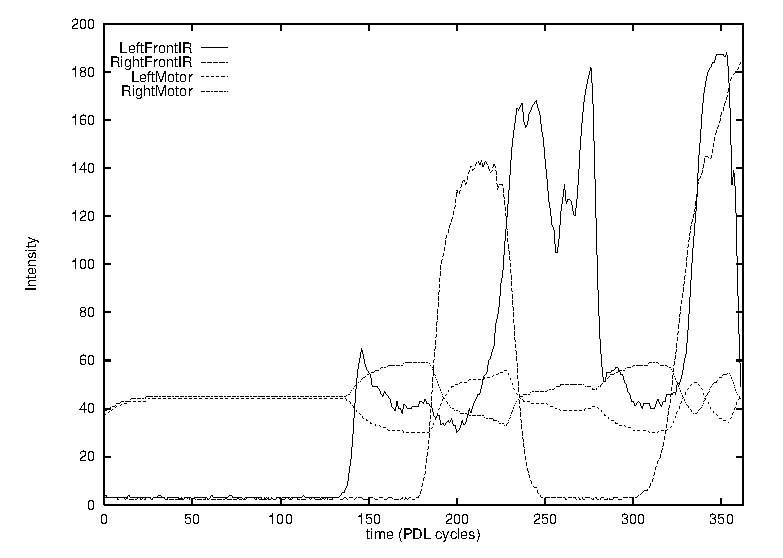
\includegraphics[width=9cm]{robots//irtaxis.eps}}
\caption{This figure shows the evolution of the infrared sensors and motor values in time during phototaxis, i.e. the emergent dynamics of combining the processes \texttt{Taxis} and \texttt{TowardsDefault}. On the x-axis the time is shown in the basic time unit of the robots, a {\sc pdl} cycle ($= \frac{1}{40} s$). The y-axis shows the intensity of the infrared sensors and motor signals. The data is taken from a robot that was driving using both processes \texttt{Taxis} and \texttt{TowardsDefault}. It drove straight forward until at time 140 the robot detected an infrared source after which it adjusted its motor signals to home in on the source.}
\label{f:irtaxis}
\end{figure}



This process causes the robot to change its speed towards a default speed with certain step size. The step size is introduced to let the robot accelerate smoothly. Note that this way the motor values do not reach the default speed; the values approach it asymptotically. When the processes are defined, the network looks like in \figref{f:robots:pdl}.

Taking the two processes together results in the emergent behaviour that the robot will move wiggling towards the infrared source (see \figref{f:irtaxis}). Such phototaxis behaviour, although with a slightly different implementation, was introduced for a robot application by Valentino \citet{braitenberg:1984} and has already been discussed extensively in the literature, see e.g. \citealt{steels:1994}.

\begin{figure}
\centerline{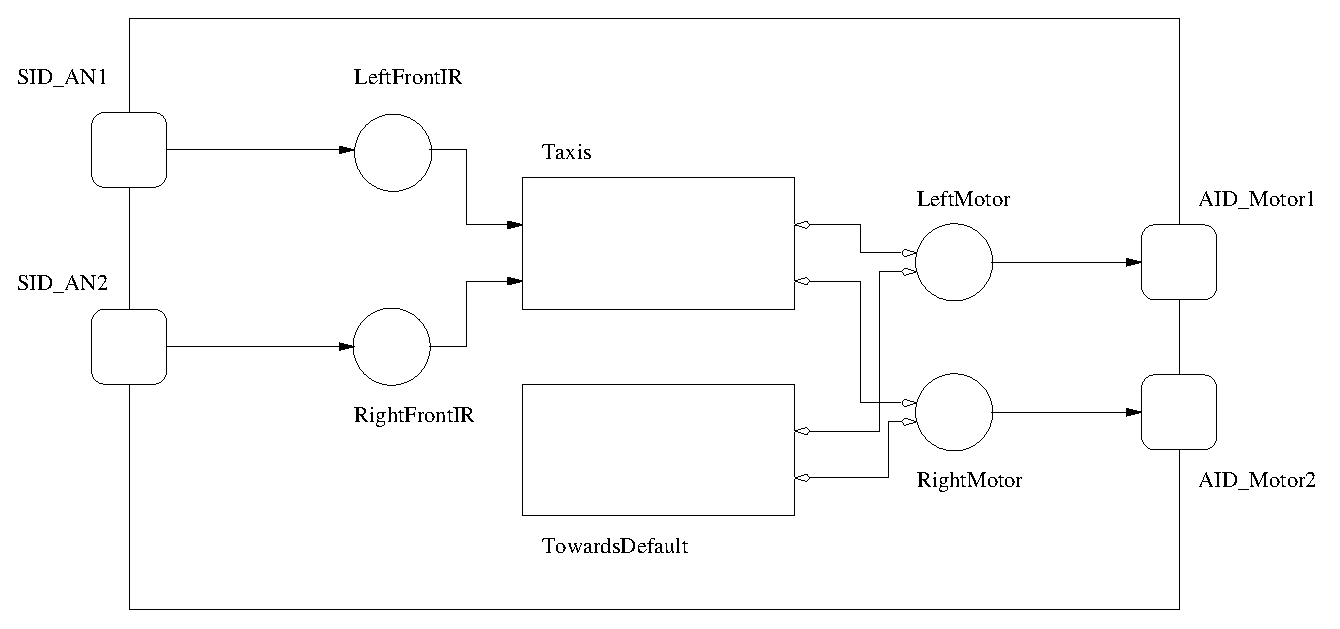
\includegraphics[width=9cm]{robots//pdl_network.eps}}
\caption{Finally the network of quantities and processes for the phototaxis example is complete. The {\ttfamily LeftFrontIR} and {\ttfamily RightFrontIR} are connected to input {\ttfamily Taxis}, which outputs to the motor quantities. The motor quantities are also used to calculate the output, hence this connection is bi-directional. The process {\texttt TowardsDefault} does not use any sensors; as in Taxis it only uses values of the quantities {\ttfamily LeftMotor} and {\ttfamily RightMotor} thus giving the bi-directional connection between {\ttfamily TowardsDefault} and the motors.}
\label{f:robots:pdl}
\end{figure}

Appendix \ref{a:pdl} presents the structure of the implemented {\sc pdl} program in more detail. In the next section the behaviour based architecture is expanded to incorporate planned behaviours as well.

\index{phototaxis|)}

\section{Cognitive architecture in PDL}\label{s:robots:architecture}
	
\index{behaviour-based!architecture}
\index{behaviour-based!cognitive architecture|(}

\begin{figure}
\centerline{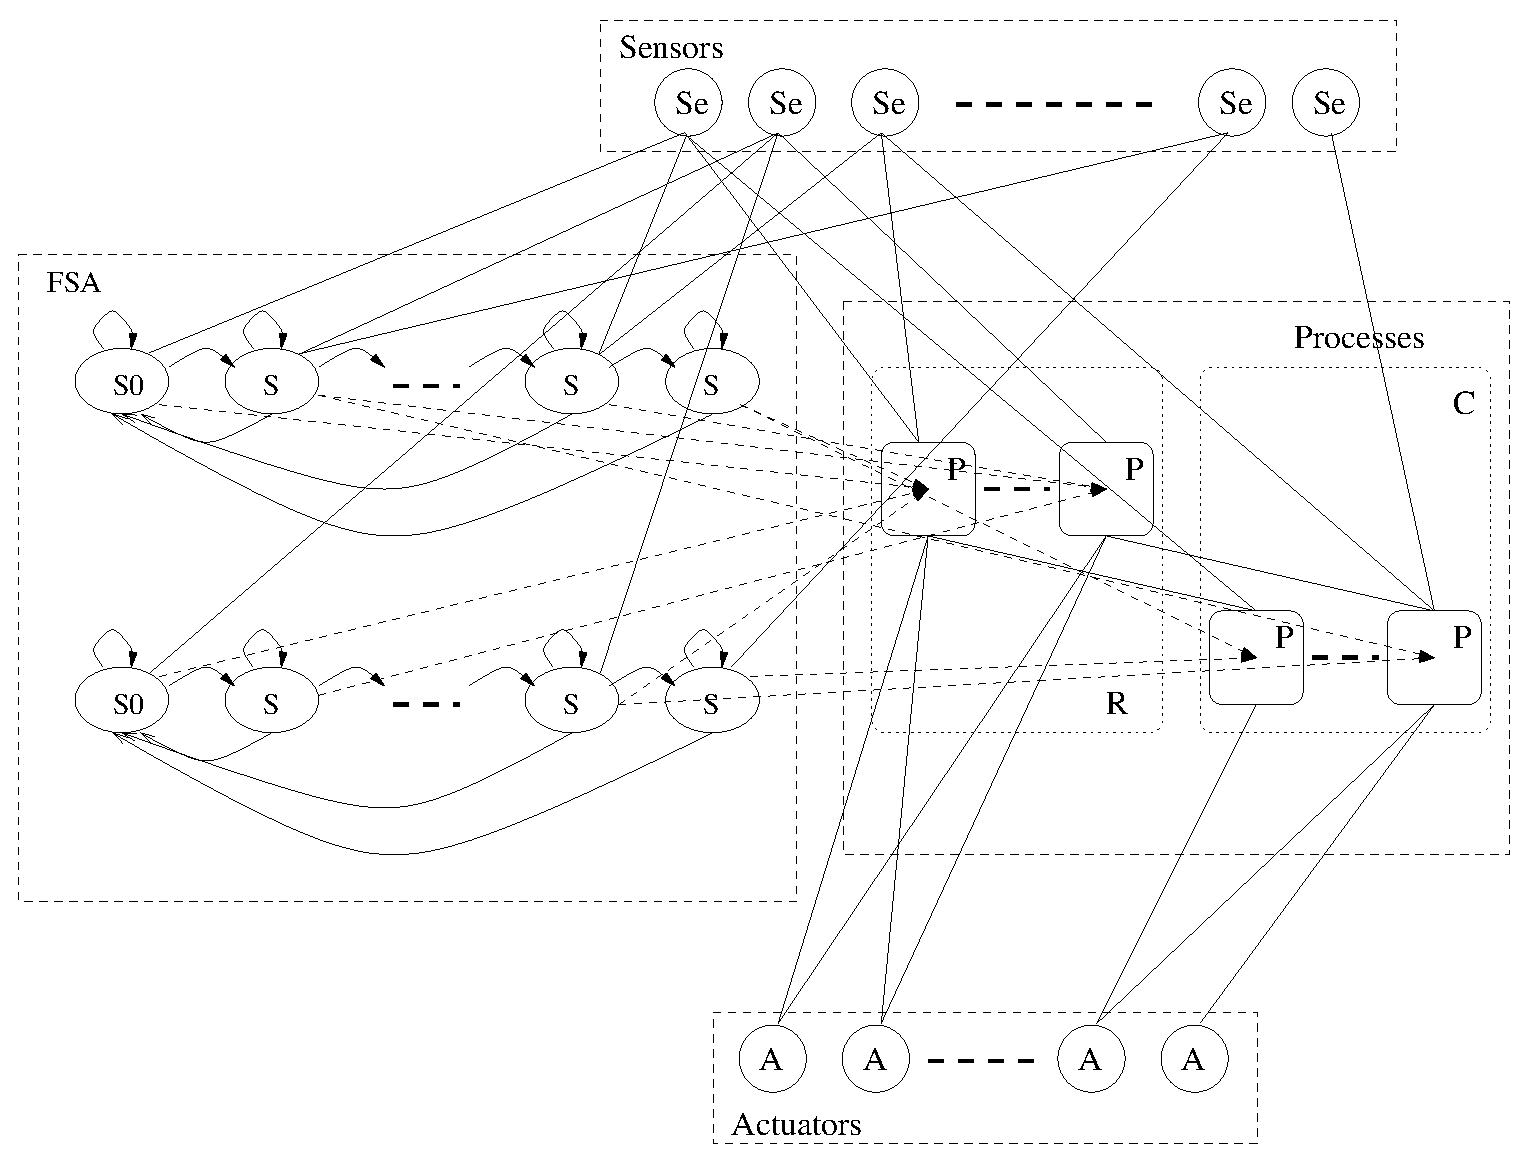
\includegraphics[width=9cm]{lang_games//fsa.eps}}
\caption{A schematic overview of the developed architecture. See the text for details.}
\label{f:architscheme}
\end{figure}

To accomplish a complex task like communication, a sequence of actions have to be planned. Reactive behaviours like phototaxis alone do not suffice. To allow the robots to execute planned behaviour a new architecture has been developed. This resulted in what could be called a {\scshape behaviour-based cognitive architecture} that is primarily based on the behaviour-based control architecture proposed by Luc \citet{steels:1994b}. This cognitive architecture could be applied as a general purpose architecture for complex and dynamic tasks like navigation. The architecture executes a script (or plan) through excitation and inhibition of processes that altogether result in some emergent behaviour. The scripts are implemented as finite state automata in which transitions are controlled by state-specific pre- and post-conditions. In each state of the finite state automaton \textsc{(fsa)} a particular set of processes are activated or inhibited. \figref{f:architscheme} shows the basic principle.

In the architecture the sensors $Se$ and actuators $A$ are coupled through a complex of connections. The agent consists of a set of scripts, which are implemented as finite state automata. The finite state automata are parallel processes where transitions are regulated by pre- and post-conditions. Usually the pre- and post-conditions are satisfied by some sensory stimuli. A state may also be fed with information coming from some internal process (not shown). Every state $S$ has a post-condition that allows the system to enter the default state $S0$ where nothing happens. Each state of the automaton has excitatory and inhibitory connections with dynamic sensorimotor processes $P$. The excitatory connections are drawn as dotted lines, the inhibitory have been left out for clarity of the picture. The processes are divided between reactive {\scshape (R)} and cognitive {\scshape (C)} processes. The reactive processes have more direct processing and can take usually only sensorimotor data as input. The cognitive processes are more complex, and may take also stimuli coming from other internal processes. Note that the finite state automaton could be considered as a cognitive process as well. The configuration of excitatory processes and the dynamics of the robot with its environment cause the robot to perform some emergent behaviour. Hence the system is consistent with the behaviour-based paradigm.

Activation of processes is modelled by invoking motivational factors (cf. \citealt{steels:1996d,jaeger:1997}). For example if is a state that in which the motivation for doing infrared taxis is present, this state may be a motivational factor \texttt{MotIRT} that is set to 1. The process taxis can then look like this:

\begin{lstlisting}
void Taxis()
{
  D=value(RightFrontIR)-value(LeftFrontIR);
  add_value(LeftMotor,MotIRT*C*F(D)*D));
  add_value(RightMotor,-MotIRT*C*F(D)*D));
}
\end{lstlisting}

A multi-agent system is a parallel process in which two robots cooperate autonomously. In order to synchronise these two parallel processes, the robots use pre-programmed radio communication. The robots playing a language game process dependent, but parallel operating finite state automata. A signal is broadcasted when both robots should transfer to another state simultaneously as the result of the transition of one of the robots.

\begin{figure}
\centering
\subfigure[Brooks]{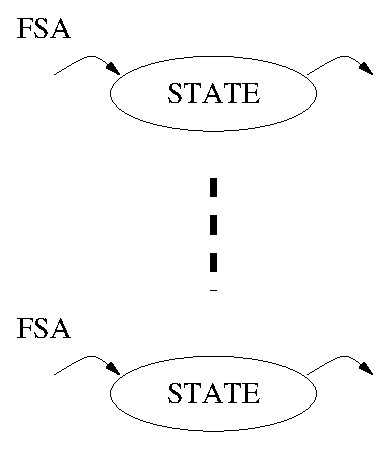
\includegraphics[width=4cm]{lang_games//fsabrooks.eps}}
\subfigure[Vogt]{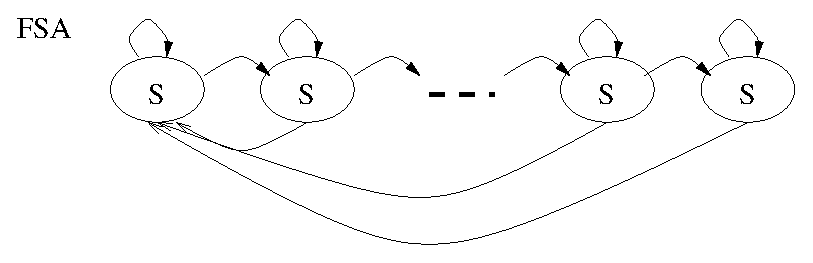
\includegraphics[width=8.5cm]{lang_games//fsavogt.eps}}
\caption{The finite state automata as used in the subsumption architecture (a) and in the cognitive architecture (b). In the subsumption architecture the finite state automata usually only has one state that models a particular behaviour. This behaviour can inhibit (or subsume) another behaviour. The cognitive architecture has some finite state automata each modelling a script-like behaviour. Each state excites or inhibits a number of dynamical processes. The finite state automata function independently as a parallel process.}
\label{f:fsa}
\end{figure}

Because the architecture uses finite state automata, readers may wrongly suggest it is the subsumption architecture proposed by Rodney \citet{brooks:1990}. In the subsumption architecture each process is viewed as a finite state automaton on its own with only one state that models a behaviour (\figref{f:fsa} (a)). The architecture proposed here uses possibly more finite state automata each with a sequence of states that can be entered (\figref{f:fsa} (b)). These finite state automata are used to control planning. A process in the cognitive architecture can be activated by several states, and a particular state can activate several processes. In addition the processes couple the sensors with the motors, like the behaviour-based architecture proposed by Luc \citet{steels:1994b}.
\index{subsumption architecture|}
\index{Brooks, Rodney|)}
\index{dual dynamics}


The behaviour-based cognitive architecture has strong similarities with the dual dynamics architecture \citep{jaeger:1997}. However, the in the dual dynamics the activation of processes is regulated internally of these processes. There is no explicit finite state automaton that regulates the activation.

\index{PDL|)}

\index{behaviour synthesis architecture}
The architecture proposed here is also similar to the architecture proposed by \citet{barnes:1996} and \citet{barnesetal:1997}, called the behaviour synthesis architecture ({\sc bsa}), which synthesises a set of {\em behaviour patterns} with a certain utility (or strength) for accomplishing a task. A {\em behaviour script} controls a sequence of {\em behaviour packets}. Each behaviour packet consists of a set of behaviour patterns, a pre-condition and a post-condition. Comparing the behaviour patterns with the dynamical processes of {\sc pdl}, the behaviour scripts with the finite state automata and the packets with a single state, then the {\sc bsa} is very close to the architecture that has been incorporated here. Main differences with the work of \citet{barnes:1996} is the use of utility functions as its synthesis mechanism. Although the architecture here is developed by a human programmer, \citet{barnesetal:1997} show that planning can be automated using the {\sc bsa}.
\index{behaviour-based!cognitive architecture|)}


\section{Summary}

In this chapter the basic set-up of the robots, their software and environment were introduced. The experiments use two small {\sc lego} vehicles that are equipped with a set of sensors, actuators, a battery pack and a specialised sensorimotor board {\sc smbii}. The robots are programmed in a specialised programming language {\sc pdl}, which is dedicated to process the dynamics of sensorimotor behaviours in the behaviour-oriented paradigm.

The principles of {\sc pdl} have been extended to a behaviour-based cognitive architecture. In this new architecture robots can execute planned behaviour as cognitive processes.

The robots as introduced here are the physical bodies with which the agents try to develop their ontologies and lexicons. How they do that is explained in \chapref{ch:lg}. As shall become clear some processing is done off-board. This is mainly done to experiment more efficiently and to be able to test different approaches on recorded data.  In some specific experiments the architecture of the robots has been changed with respect to the description given in this chapter. Relevant changes will be reported when these experiments are discussed.

More detailed information on the {\sc pdl} program can be found in Appendix \ref{a:pdl}.